\chapter{Project 6: Web}

\section{Overview}
There's one piece of hardware that we haven't talked about yet. The ESP32-C3 microcontroller has a
WiFi processor built in. We can make use of this to connect to the internet and pull in all kinds of
data or transmit data to other services! If you've ever heard the phrase "Internet of Things", this
is what they mean. Over the course of this project, you will:
\begin{itemize}
    \item Use the embedded WiFi processor to connect to the internet
    \item Make requests to free 3rd party API services to fetch live data
    \item Use the connected buttons and screen to display different sets of that data
\end{itemize}
At the end of this project, your microcontroller should run a MicroPython program that displays 3
different screens of data that you can rotate through with the buttons. Let's get started!
\begin{figure}[H]
\centering
    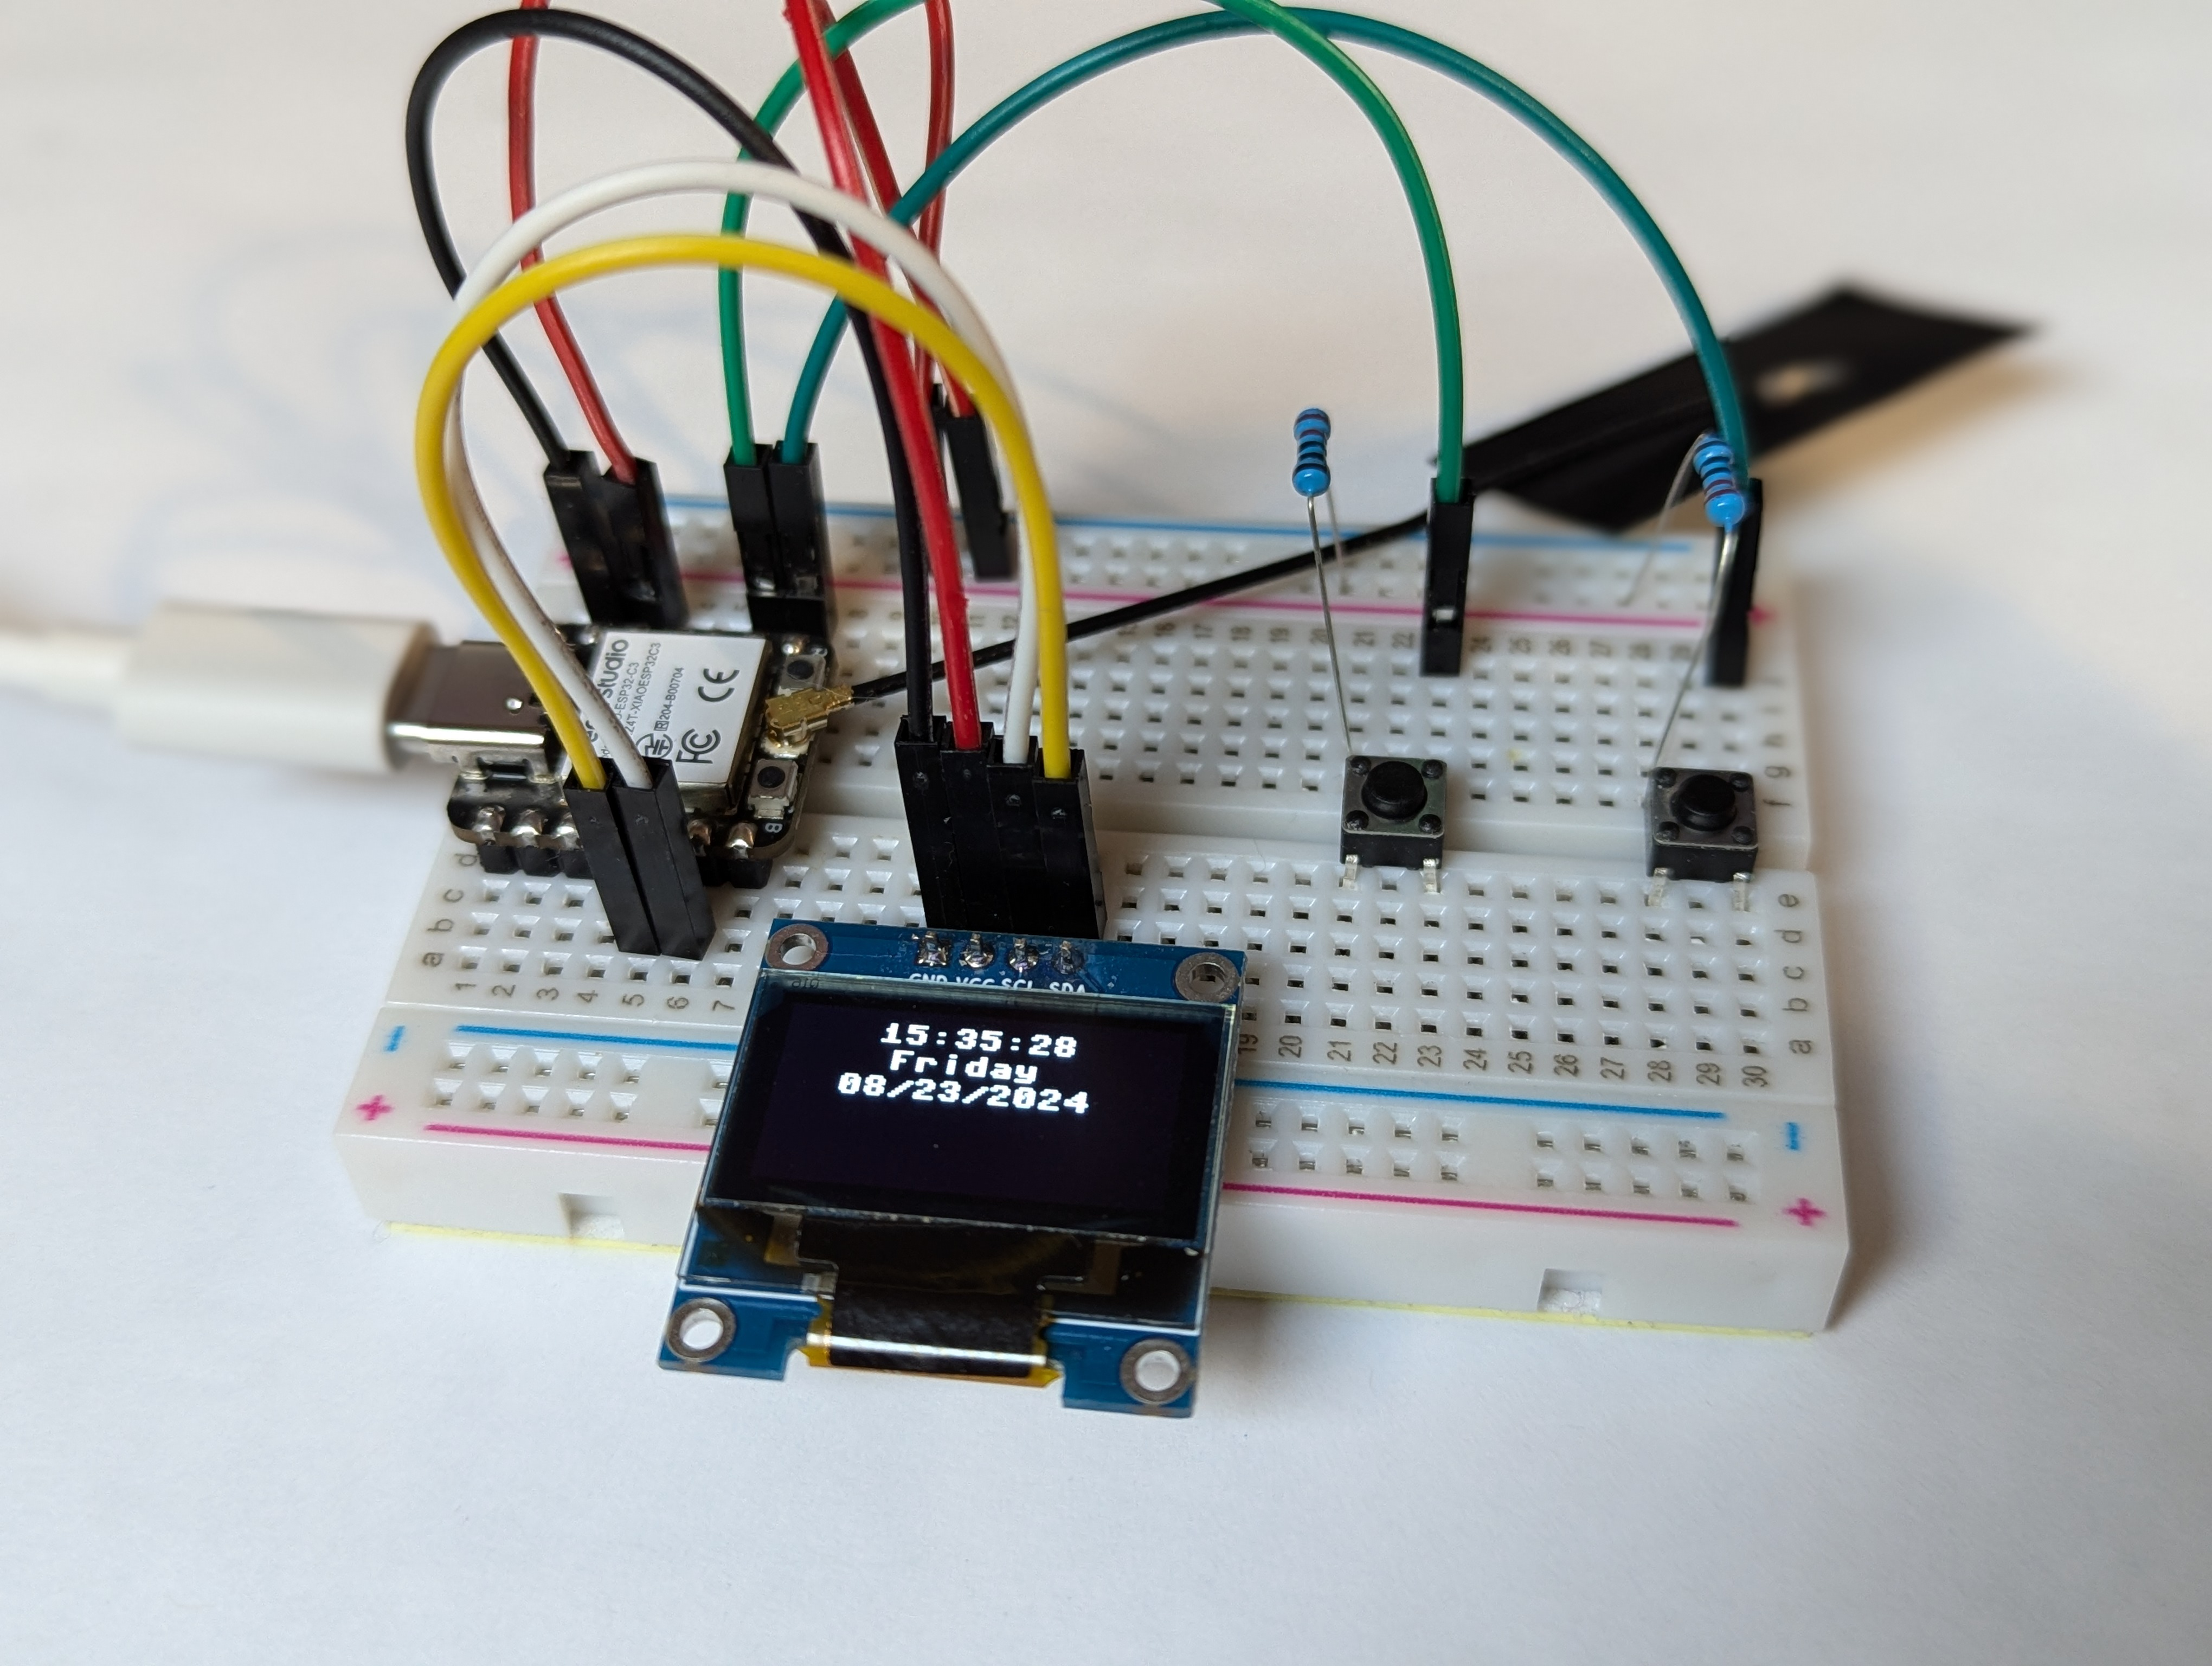
\includegraphics[width=.6\linewidth]{chapter_6/screen_connected.jpg}
    \caption{The end result should look something like this}
\end{figure}

\pagebreak

\section{Directions}

\subsection{Creating the circuit}
Using jumper cables, you will be assembling a circuit between your microcontroller, your breadboard, two
buttons and the small OLED screen included in your kit.

\subsubsection{Remove previous components}
Before beginning, remove any components from prior chapters including LEDs, buttons, and wires. You may leave the
microcontroller attached to the breadboard.

\subsubsection{Attach the microcontroller to the breadboard}
If it's not already, carefully insert the pins at the bottom of your microcontroller into the breadboard. Refer back
to \ref{pinout} for pin labels. When placing the board into the breadboard, make sure that the microcontroller is oriented such that:
\begin{itemize}
    \item The pin labeled \textbf{5V} is inserted in hole at \textbf{Column H, Row 1} of the breadboard (or \textbf{H1}, for short)
    \item The pin labeled \textbf{GPIO2} is inserted in hole \textbf{D1} of the breadboard
    \item The pin labeled \textbf{GPIO20} is inserted in hole \textbf{H7} of the breadboard
    \item the pin labeled \textbf{GPIO21} is inserted in hole \textbf{D7} of the breadboard
\end{itemize}
You may need to apply more pressure than expected to seat the microcontroller properly in the breadboard. When its over, it should look like this:
\begin{figure}[H]
    \centering
    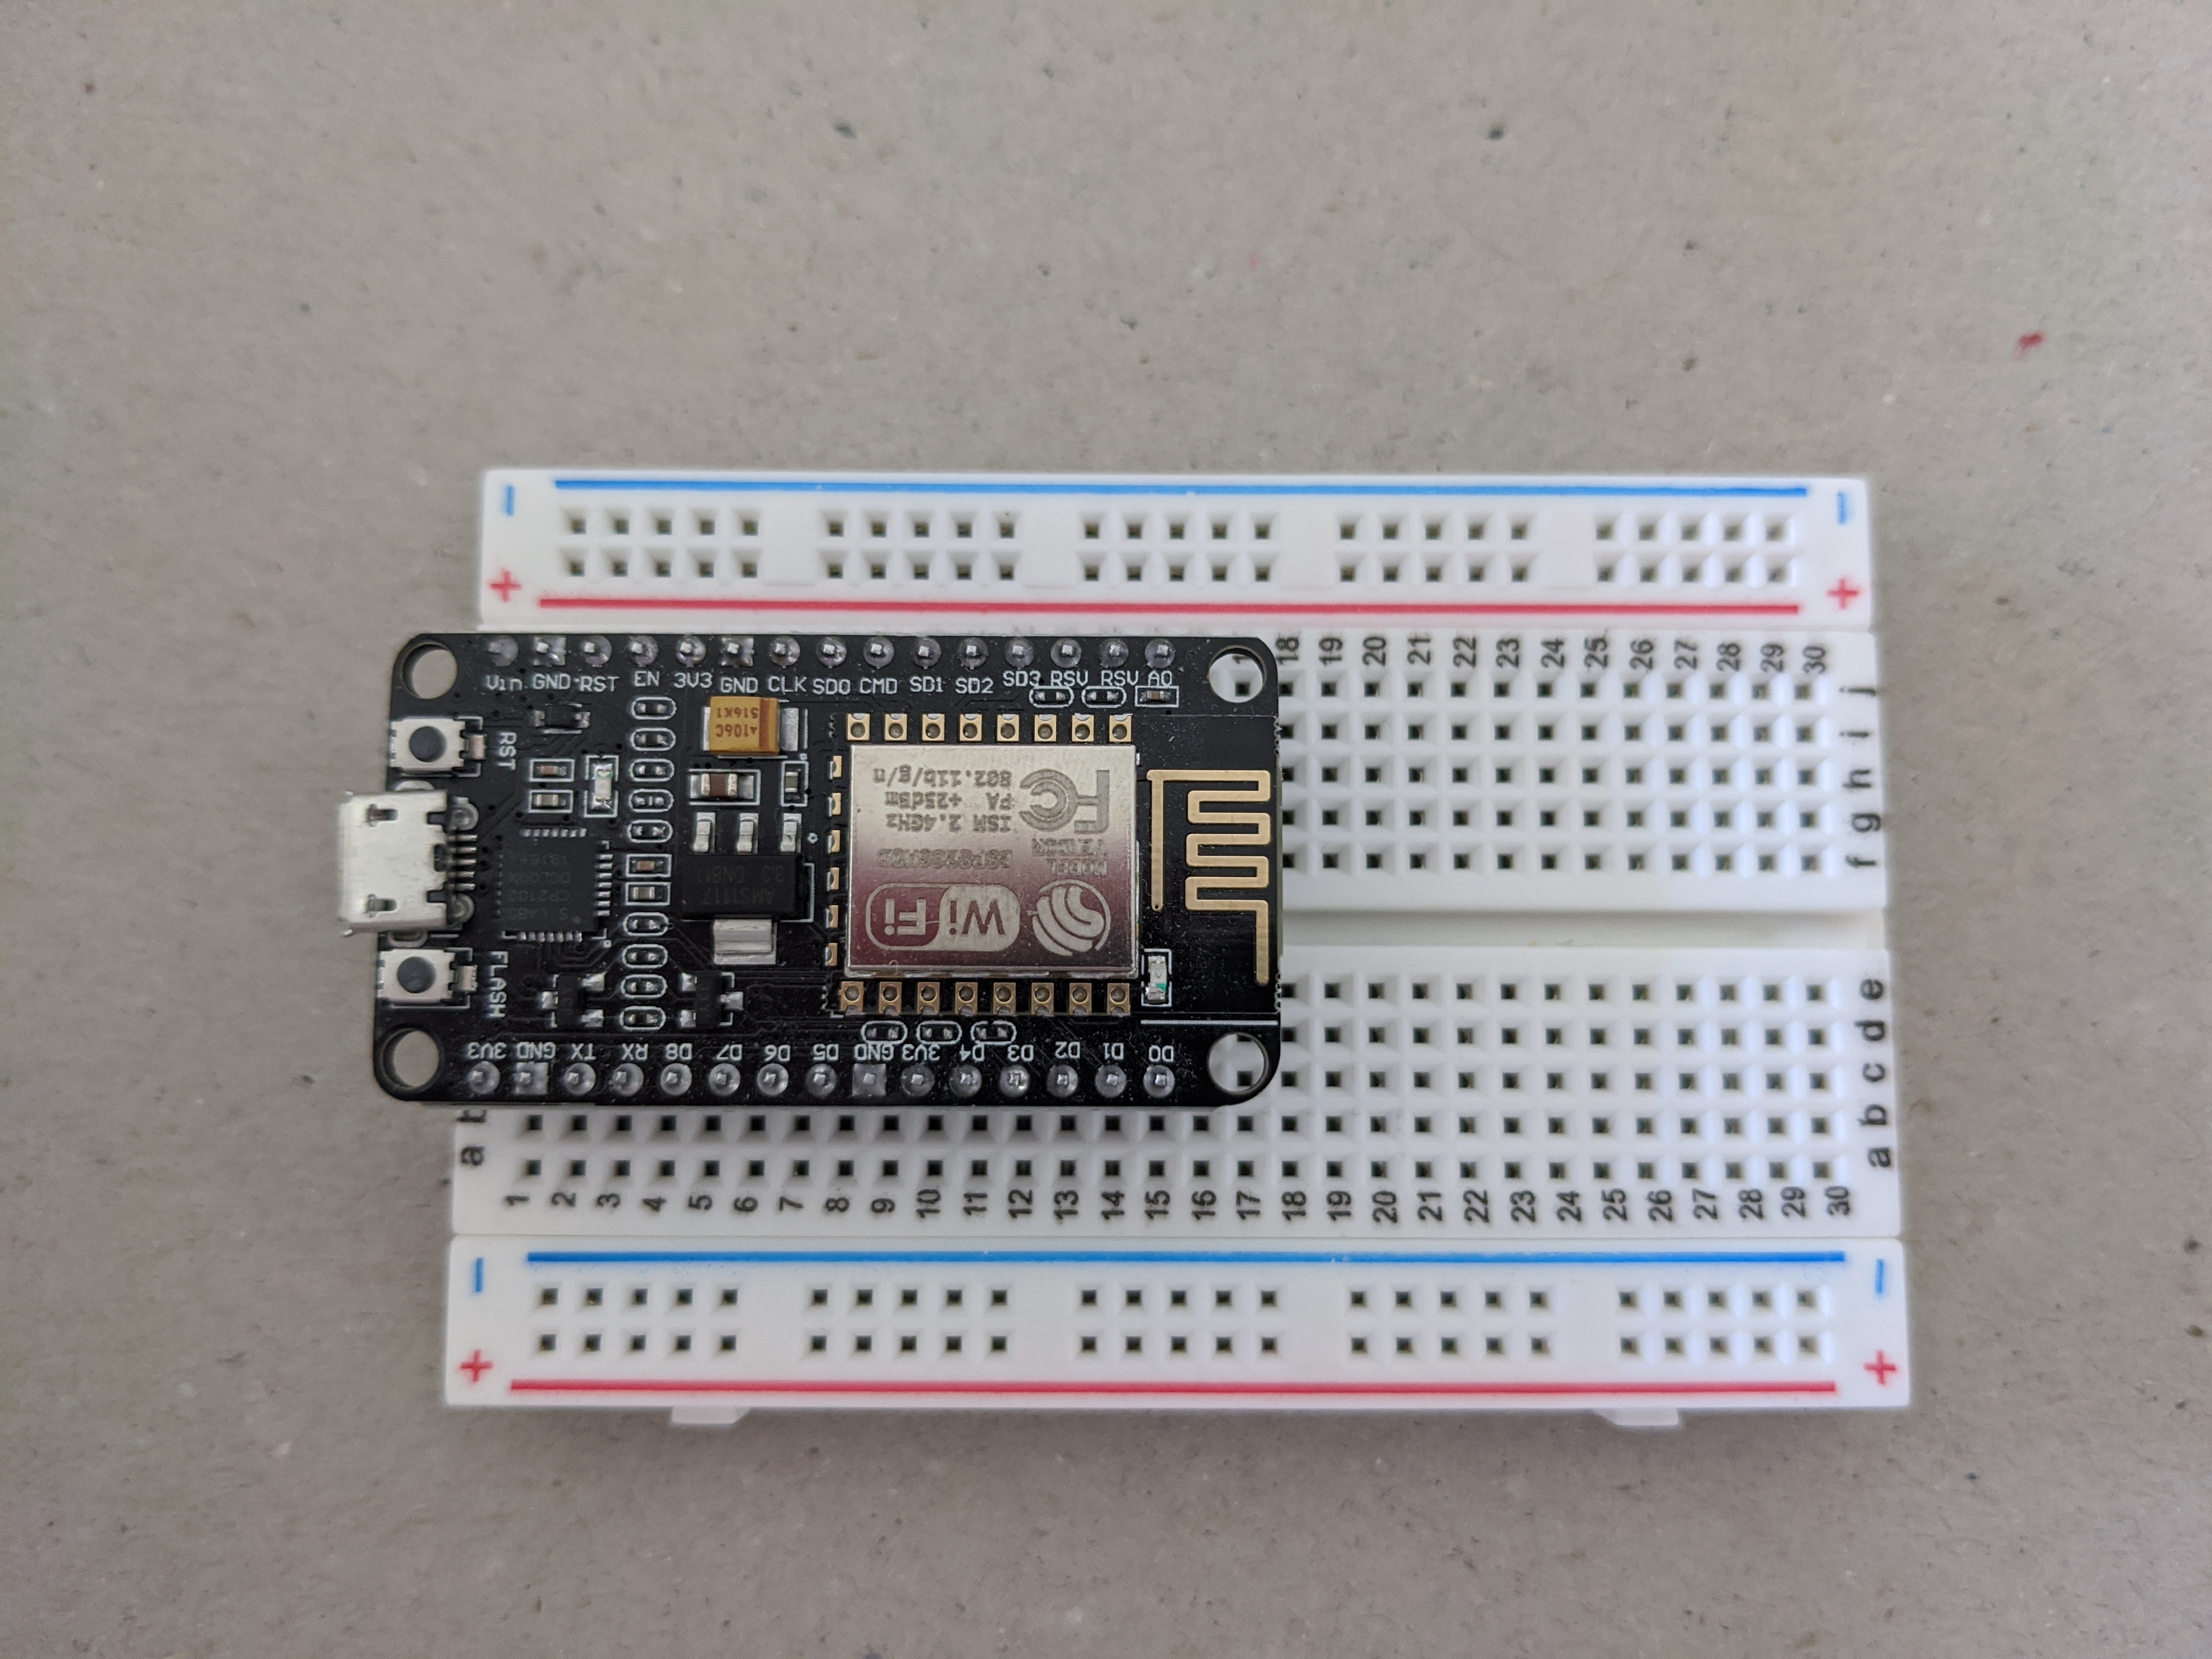
\includegraphics[width=.6\linewidth]{common/microcontroller_seated_in_breadboard.jpg}
    \caption{So far, so good!}
\end{figure}

% more content to come
